\section{Tests and Results}
\label{chap:Tests and Results}

This section first provides details about the implementation and the used instances. Thereafter the results are described and interpreted.




This situation has some problems. Trailers will still incur their fixed costs even though de facto no trailer is used. Furthermore, this usage of trailers reduces the amount of available trailers that can be used as actual trailers. To resolve this issue, synthetic trailers are added to the model without fixed costs, with infinite distance costs per distance unit and an infinite capacity to function as unloading docks for the lorries.
These trailers will never be used as actual trailer due to their distance costs.
% Therefore the costs incurred by a lorry that uses such a synthetic trailer as unloading dock are the time that it takes to couple and decouple at the depot.
\\

In the VRPTT these synthetic trailers don't have an impact on the best found solutions.
If a lorry would couple such a synthetic trailer, it will have to be the first event on its path after starting its path.
After coupling the trailer the lorry will either move away from the depot and incur infinite distance costs or go to the synthetic trailer's decouple vertex after which the lorry will have to end its path without having contributed at all to the collection of customer supply.


\subsection{Instances}



Drexl has created a set of VRPTT test instances  in \cite{drexl2014bandc}   structured to resemble the situation in raw milk collection.
These use two lorry and two trailer classes as specified in Table \ref{tab:vehpar}.
Enough vehicles of each class are included such that all of the customer's supply can be collected with either only class 1 lorries and class 2 trailers, or class 2 lorries and class 1 trailers.
The synthetic trailer class is added to instances to facilitate multiple unloads.
They are not part of Drexl's instances.
For each customer in an instance a synthetic trailer is added.
\\

% The synthetic trailer class is added to facilitate multiple unloads.

 % but are of no consquence for the results to the VRPTT.






 Trailers will still incur their fixed costs if they are used as unloading docks, even though de facto no trailer is used. Furthermore, using a trailer as unloading dock reduces the amount of available trailers that can be used as actual trailers.
 To resolve these two issues, synthetic trailers without fixed costs, with infinite distance costs per distance unit and an infinite capacity are added to the fleet of the instances.
 % s many synthetic trailers as there are customers.
 % These instances can then function as unloading docks for the lorries.
These trailers will never be used as actual trailer due to their distance costs.
% Therefore the costs incurred by a lorry that uses such a synthetic trailer as unloading dock are the time that it takes to couple and decouple at the depot.
In the VRPTT these synthetic trailers don't have an impact on the best found solutions.
If a lorry would couple such a synthetic trailer, it will have to be the first event on its path after starting its path.
After coupling the trailer the lorry will either move away from the depot and incur infinite distance costs or go to the synthetic trailer's decouple vertex after which the lorry will have to end its path without having contributed at all to the collection of customer supply. \\




\begin{table}[h]
\caption{Vehicle Parameters}
\label{tab:vehpar}
\hspace*{-3.5cm}\begin{tabular}{lllllllll}
\toprule
Vehicle  & Number  & Fixed  &  Cost  &  Cost  &  Capacity &  Driving speed & Driving speed  & Load transfer time in  \\
 class & of axles & cost &   per km &   per hour &   &  short distance & long distance & minutes per 1000 units \\
 \midrule
%------------------------------------
Lorry 1 &2 &180 &0.65 &36 &10000& 25 &65 &2 \\
Lorry 2 &3 &200& 0.70& 36& 15000& 25 &65 &2\\
Trailer 1 &2& 20& 0.04& 0 &10000 &25 &65 &\\
Trailer 2 &3 &25 &0.06 &0 &15000& 25& 65 &\\
Synthetic & 2 & 0 & $\infty$ & 0 & $\infty$ & 25 & 65 & \\
Trailer & & & & &&& &\\
%----------------------------------------
\bottomrule
\end{tabular}
\end{table}


The customer and transshipment locations are randomly selected on a 100 by 100 kilometer grid with the depot located in the center.
The distances between the vertices is equal to the euclidean distances increased by 30 \% and rounded up the nearest integer.
%
The amount of customer supplies are chosen randomly from the interval $[1000 , 10000]$ such that even the smallest vehicle can hold the whole supply of any customer.
%
% As load transfer time, 2 min per 1,000 units of supply are
The instances have a planning horizon of 1320 minutes.
The time window of each location is equal to the whole planning horizon, hence the interval [0,1320].
These nonrestrictive time windows correspond to
the situation in raw milk collection where  few
customers or transshipment locations have time windows. \\

%
With these parameters, 30 instances
were created per instance size, where the instance size varied between two and 25 customers.
% with two, four, six and eight customers.
%
% denoted by x\_y\_z\_n, where $2 \leq x \leq 8$ stands for the number of
% customers, $2 \leq y \leq 8$ for the number of transshipment locations,
% $ z \geq 4 $ for the number of vehicles and
% $ 0 \leq n \leq 30$ is the index of the instance type.
%
The amount of transshipment locations is always equal to the amount of customers.
Half of the customers consist of trailer customers, the other half of lorry customers.
Half of the transshipment locations consist of trailer customers, the other half of pure transshipment locations.
%
\\

The cut-off distance $\phi $ is five kilometers.
%
The duration of visiting a transshipment vertex $\tau^{\rm R}$ is five minutes.
%
The values used for time and distance are nonnegative integers.
In a note accompanying the instances Drexl describes that the travel time in minutes between a pair of vertices is computed by dividing the distance by the driving speed and multiplying it by 60. Only then should the value be rounded off to the nearest integer.
\\
% assumed.

% Two sets test instances and bounds are used to benchmark this thesis' model and VNS: which can be used to compare the results of this thesis' method with are provided in   \cite{drexl2014bandc} and \cite{drexl2011branch}.


\subsection{Bounds}
Upper bounds (VRPTT\_UB) and lower bounds (VRPTT\_LB)  on the minimum costs for the VRPTT are provided in ~\cite{drexl2014bandc} for instances with up to eight customers.
For all instances with two and four customers, the optimal value was found.
 % for 120 test instances with up to eight customers.
 The cost function that is used in ~\cite{drexl2014bandc} excludes time related costs, i.e., the bounds are on the sum of the fixed and the distance costs.
Optimal values for the truck and trailer routing problem (TTRP) for the instances used in ~\cite{drexl2014bandc} are provided in \cite{drexl2011branch}. These values are referred to as TTRP\_OPT. The costs function that is used in \cite{drexl2011branch} includes time related costs.  The TTRP is a special version of the VRPTT, where trailers are not allowed to be shared, i.e., a trailer can not be decoupled by one lorry and coupled again by another lorry.
%
The values of the bounds and the values found by the VNS are all included in Appendix \ref{sec:bounds}.


\subsection{Implementation Details }
%TODO although I've tried to folllow Drexl's instruction on rounding, I didnt end up with the same numbers. I'm fairly certain that on the small instances we have the same sol, but not same costs. Error is equally distr around hsi value so no sytematic help.. also in the figure you see that the lines follow each other quite good.

% The division of Length by Speed must be double precision, not integer, i.e., the division of 60 by 65 must return 0.923..., not 0






The results reported in this section were obtained by running the optimization method three times.
% with and without constraint (\ref{con:extra}).
The algorithm was stopped after three minutes or 3000 iterations, whichever came first.

In Table \ref{tab:parameters}  the used parameters are given.
These parameters were found to be effective without performing a hyperparameter optimization, so better parameters can probably be found.


The maximum flow algorithm that is used to calculate the load table is the push-relabel algorithm   \cite{goldberg1988new}.
The longest path algorithm that is used to calculate the time table is the Floyd-Warshall algorithm \cite{Floyd}


\begin{table}[ht]
\centering
\caption{Method parameters}
\label{tab:parameters}
\begin{tabular}{ll}
\toprule
Parameter       & Value       \\ \midrule
%
$\tau^{\rm D}$ & 0 \\
$p$   & 0.2    \\
$nSamples $ & 10 \\
$\eta$ & 3 \\
$\omega^{\rm unserved-customer}$ & 40000 \\
$\omega^{\rm lorry-customer}$    & 20000 \\
$\omega^{\rm time-window}$       & 2 \\
$\omega^{\rm capacity-shortage}$ & 4 \\
%
%  $\{1,2\}$                        \\ \hline
% Lorry class 2   & 15000                & 200    & 0.7        & 65            & $\{1\}$                          \\ \hline
% Trailer class 1 & 10000       & 20     & 0.04       &               &  $\{1,2\}$                          \\ \hline
% Trailer class 2 & 15000          & 25   & 0.04          &               &   $\{1\}$                         \\ \hline
\bottomrule
\end{tabular}
\end{table}

\subsection{Results}


In this subsection we interpret the results found by the VNS.
The time related cost are included when the solutions found by the VNS for the VRPTT and VRPTTMU are compared with the TTRP\_OPT and excluded when compared with the VRPTT\_LB and VRPTT\_UB.
% are compared with the values found by the VNS for the VRPTT and the VRPTTMU.
% The time related cost are excluded when the bounds on the VRPTT, VRPTT\_LB and VRPTT\_UB, are compared with the values found by the VNS for the VRPTT and the VRPTTMU.
 For each instance the available bounds and the values found by the VNS are plotted in Figure \ref{fig:single_unload}.
Statistic of the gaps between the values found by the VNS and the available bounds are given in Table \ref{tab:gaps}

 \begin{figure}[!h]
   % \hspace*{-1.5in}
     \centerline{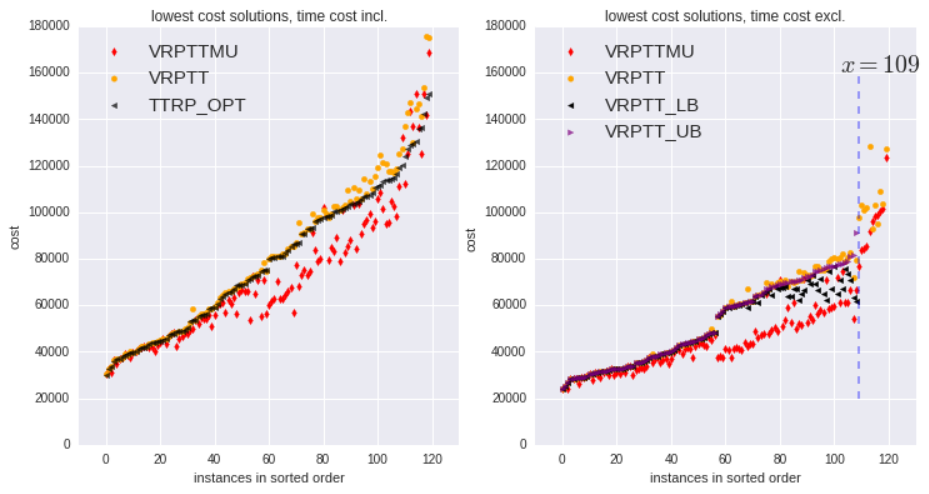
\includegraphics[width=1.3\textwidth]{img/results_1fig.png}}
   \caption{
   The lowest cost found by the VNS for each instance with the available bounds.
   The left plot excludes time cost.
   Its instances are sorted such that the values of TTRP\_OPT increase monotonically.
   The plot on the left includes time cost.
   Its instances are sorted such that all 109 known values of VRPTT\_UB increase monotonically. }
   \label{fig:single_unload}
 \end{figure}


 \setlength\LTleft{-1.3in}
 \setlength\LTright{-1in}
 % \noindent\makebox[]\linewidth]{
 \begin{longtable}{lrrcrrcrr}
   % \\
   \newpage
 \toprule
 % & \multicolumn{2}{c}{time costs included} & \phantom{a}& \multicolumn{4}{c}{excluding time costs} \\
 & \multicolumn{2}{c}{TTRP\_OPT, time cost incl.} & \phantom{a}& %\multicolumn{4}{c}{excluding time costs} \\
 \multicolumn{2}{c}{VRPTT\_LB, time cost excl.}&\phantom{a} & \multicolumn{2}{c}{VRPTT\_UB, time cost excl.} \\
 \cmidrule{2-3} \cmidrule{5-6} \cmidrule{8-9}
  &  VRPTT &  VRPTTMU &&  VRPTT &  VRPTTMU & & VRPTT &  VRPTTMU \\
 \midrule
 %
 2 customers \\
 \cmidrule{1-1}
 count &                30.0 &                  30.0 &&                 30.0 &                   30.0 &&                 30.0 &                   30.0 \\
 mean  &                 0.0 &                  -3.5 &&                 -0.0 &                   -4.5 &&                 -0.0 &                   -4.5 \\
 std   &                 0.6 &                   4.9 &&                  0.1 &                    4.8 &&                  0.1 &                    4.8 \\
 min   &                -1.3 &                 -17.6 &&                 -0.3 &                  -16.0 &&                 -0.3 &                  -16.0 \\
 % 25\%   &                -0.7 &                  -5.7 &&                 -0.0 &                   -8.1 &&                 -0.0 &                   -8.1 \\
 % 50\%   &                 0.4 &                  -1.1 &&                  0.0 &                   -2.3 &&                  0.0 &                   -2.3 \\
 % 75\%   &                 0.4 &                   0.4 &&                  0.0 &                    0.0 &&                  0.0 &                    0.0 \\
 max   &                 0.6 &                   0.6 &&                  0.0 &                    0.0 &&                  0.0 &                    0.0 \\
 \\
 %
 4 customers \\
 \cmidrule{1-1}
 count &                30.0 &                  30.0 &&                 30.0 &                   30.0 &&                 30.0 &                   30.0 \\
 mean  &                 0.7 &                 -10.5 &&                  0.1 &                  -13.8 &&                  0.1 &                  -13.8 \\
 std   &                 1.6 &                  10.1 &&                  0.8 &                   12.8 &&                  0.8 &                   12.8 \\
 min   &                -0.8 &                 -34.2 &&                 -0.4 &                  -37.0 &&                 -0.4 &                  -37.0 \\
 % 25\%   &                 0.4 &                 -21.0 &&                 -0.1 &                  -29.4 &&                 -0.1 &                  -29.4 \\
 % 50\%   &                 0.5 &                  -5.4 &&                 -0.1 &                   -7.0 &&                 -0.1 &                   -7.0 \\
 % 75\%   &                 0.7 &                  -3.2 &&                  0.0 &                   -4.0 &&                  0.0 &                   -4.0 \\
 max   &                 9.0 &                   0.6 &&                  3.6 &                    0.0 &&                  3.6 &                    0.0 \\
 % \pagebreak
 \\
 6 customers\\
 \cmidrule{1-1}
 count &                30.0 &                  30.0 &&                 30.0 &                   30.0 &&                 30.0 &                   30.0 \\
 mean  &                 1.5 &                 -12.9 &&                  3.3 &                  -18.3 &&                  1.0 &                  -20.0 \\
 std   &                 2.3 &                   7.5 &&                  4.3 &                   10.6 &&                  2.0 &                   10.7 \\
 min   &                -0.5 &                 -24.5 &&                 -0.2 &                  -32.9 &&                 -0.4 &                  -32.9 \\
 % 25\%   &                 0.2 &                 -19.4 &&                 -0.0 &                  -27.1 &&                 -0.0 &                  -28.2 \\
 % 50\%   &                 0.7 &                 -13.0 &&                  1.4 &                  -20.6 &&                 -0.0 &                  -23.8 \\
 % 75\%   &                 1.9 &                  -7.5 &&                  5.0 &                   -7.5 &&                  1.2 &                   -7.5 \\
 max   &                 9.5 &                   4.7 &&                 15.8 &                    5.0 &&                  9.6 &                    2.5 \\
 \\
 8 customers \\
 \cmidrule{1-1}
 count &                30.0 &                  30.0 &&                 19.0 &                   19.0 &&                 19.0 &                   19.0 \\
 mean  &                 6.2 &                  -5.2 &&                 13.5 &                   -9.2 &&                  0.6 &                  -19.7 \\
 std   &                 4.8 &                   9.9 &&                  7.4 &                   12.9 &&                  5.0 &                    9.2 \\
 min   &                 0.5 &                 -19.0 &&                  2.9 &                  -25.4 &&                -12.6 &                  -33.3 \\
 % 25\%   &                 2.4 &                 -13.9 &&                  7.1 &                  -18.8 &&                 -0.2 &                  -26.7 \\
 % 50\%   &                 5.9 &                  -6.0 &&                 13.0 &                  -13.8 &&                  1.7 &                  -23.0 \\
 % 75\%   &                 8.0 &                   0.4 &&                 19.7 &                    0.4 &&                  3.6 &                  -14.2 \\
 max   &                17.9 &                  15.8 &&                 28.8 &                   13.3 &&                  5.5 &                   -0.8 \\
 \bottomrule
 \\
 \caption{Statistic per instance size of the gaps between the available bounds and the lowest cost solutions found by the VNS for the VRPTT and VRPTTMU.
}
 \label{tab:gaps}
 \end{longtable}


\subsubsection{VRPTT}

% point 0: probably point 1, one of the brst solutions used trailer sharing. Give simple example with same parameters that does result in optimal solution with trailer sharing. Also critisize why this set should not be used for vrptt.
% point 1: differnce becuase of rounding; see smaller instances up to 4 customers is optimal value.. high prob of having found optimal value.  difference small. Although I followed the described rounding method I have not been able to find exactly the same values. The differences that are present are due to rounding errors. See smaller instances. average gap 0 . Perhpas mixing minutes hours and differnt metohds of rounding
% point 2: weird that vrptt always higher than ttrp.
% point 3: $ttrp < vrptt$ becuase bad algo or becuase bad instance. probably latter since vrptt not higher than vrptt\_UB.
% ALSO: use the figure to make point that follows:
%  See gap wrt to ub vrptt notime compared to gap ttrp for each instance. Are there any instances where there is a high gap with vrptt but small gap with ttrp. If so, there might be evidence that htat is a instance where sharing could be beneficial.
% point 4: examples (in txext) of instances that would have benefited from trailer sharing.\\

%from here ------------------------------------------------
In Table \ref{tab:gaps} we see that for one of the instances with two customers the VNS found a solution for the VRPTT that has a gap of -0.3 \% with the lower bound of the VRPTT, which should not be possible.
For instances with only two customers, where the probability of the VNS finding the optimal solution is the greatest, the mean and the standard deviation of the gap with the optimal value of the VRPTT is 0.0 \% and 0.1 \% respectively and with the optimal value of the TTRP 0.0 \% and 0.6 \% respectively.
The reason for this error is unknown, but at least there is evidence that the mean of the error is zero. \\


Surprisingly, for none of the instances did the best solution use trailer sharing.
This is the reason that in Figure \ref{fig:single_unload} none of the values found by the VNS are significantly lower than the optimal values of the TTRP.
All negative gaps between the values found by the VNS for the VRPTT and the optimal value of the TTRP must thus be attributed to the aforementioned error and not to the benefit of being able to share trailers. \\

Since the results for the VRPTT described in \cite{drexl2014bandc} exclude time related costs and the results for the TTRP described in \cite{drexl2011branch} include time related costs, no conclusions can be drawn about whether sharing trailers leads to solutions with lower costs on these instances based on these results alone.
Only an indirect comparison of these values can be made by using the results found by the VNS.
If sharing trailers leads  to lower cost solutions on these instances,  there may be many instances for which the gap with the upper bound of the VRPTT is significanlty greater than the gap with the optimal value of the TTRP.
In Figure  \ref{fig:gapvsgap} the gap with respect to the optimal value of the TTRP is  plotted against the gaps with respect to the bounds of the VRPTT for each instance.
The figure does not support the conclusion that trailer sharing leads to significantly lower costs on these instances.
In Table \ref{tab:gaps} we see that the mean gaps for instances with two, four, six and eight customers of the VRPTT with respect to the lower bound of the VRPTT  are 0.0, 0.1, 3.3 and 13.5 \% respectively and with respect to the upper bound 0.0, 0.1, 1.0, 0.6 \% respectively.
Therefore, the benefit of sharing trailers can not be ruled out, but can not be shown to be definitely present either.

\begin{figure}[!ht]
  \centering
    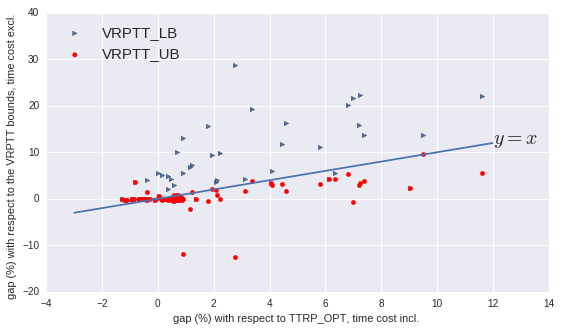
\includegraphics[width=1.0\textwidth]{img/gapvsgap.png}
  \caption{For each instance the gap with respect to the TTRP optimum against the gap with respect to the bounds of the VRPTT. }
  \label{fig:gapvsgap}
\end{figure}


The VNS was able to find solutions for all instances including the eleven instances for which no VRPTT bounds were available.


%
%
%
% a
% Surprisingly, for each instance the best found solution did not use trailer sharing.
% This is reflected in Table \ref{tab:gaps} we see that on the instances
% In Figure \ref{fig:single_unload}
% we see that for all instances the TTRP\_OPT is lower than or equal to the solutions found for the VRPTT.  This is unexpected, since we strange since it is expected that
%
% none of the instances  could our method find a solution that has lower costs than the optimal solution of the TTRP. On average our solution with the lowest cost is $2.1 \%$ more expensive than the optimal solution of the TTRP. Detailed results can be found in Appendix \ref{sec:appendix} This is surprising because one would expect that by sharing trailers between lorries, cost could be reduced. There are two posssiblities.
%  Either on these instances sharing trailers does not reduce costs, or our method could not find those solutions. \\
%
%  When we look at the results in Figure \ref{fig:single_unload} that exclude time related costs we see that for many instances no bounds are known. Our method does find solution for all instances. Our best solution is on average $3.3 \%$ more expensive than the lower bound and $0.4 \% $ more expensive than the upper bound. This gives reason to doubt whether being able to share trailer can reduce costs on these instances.


 \subsubsection{VRPTTMU}

The difference between the VRPTT and the VRPTTMU is that the latter allows lorries to do multiple trips by allowing it to visit the depot multiple times to couple a trailer, decouple a trailer or unload whereas the former does not.
In Figure \ref{fig:single_unload} we can see that for many instances the VNS finds solutions with significantly lower costs than than the TTRP and the VRPTT.
This is not surprising since in some instances less vehicles can be used, which results in less fixed costs.
The instances have such nonrestrictive time windows that one lorry can visit many customers interleaved with depot visits. \\

In Table \ref{tab:gaps} we see that for instances with two, four, six and eight customers the mean gaps with respect to the optima of the TTRP are -3.5, -10.5, -12.9 and -5.2 respectively and with respect to the lower bounds of the VRPTT -4.5, -13.8, -18.3 and -9.2 \% respectively.
This indicates that significant cost reductions can be achieved by allowing lorries to do multiple trips.
For each instance the VNS found a solution to the VRPTTMU. \\

\begin{figure}[!ht]
  \centering
    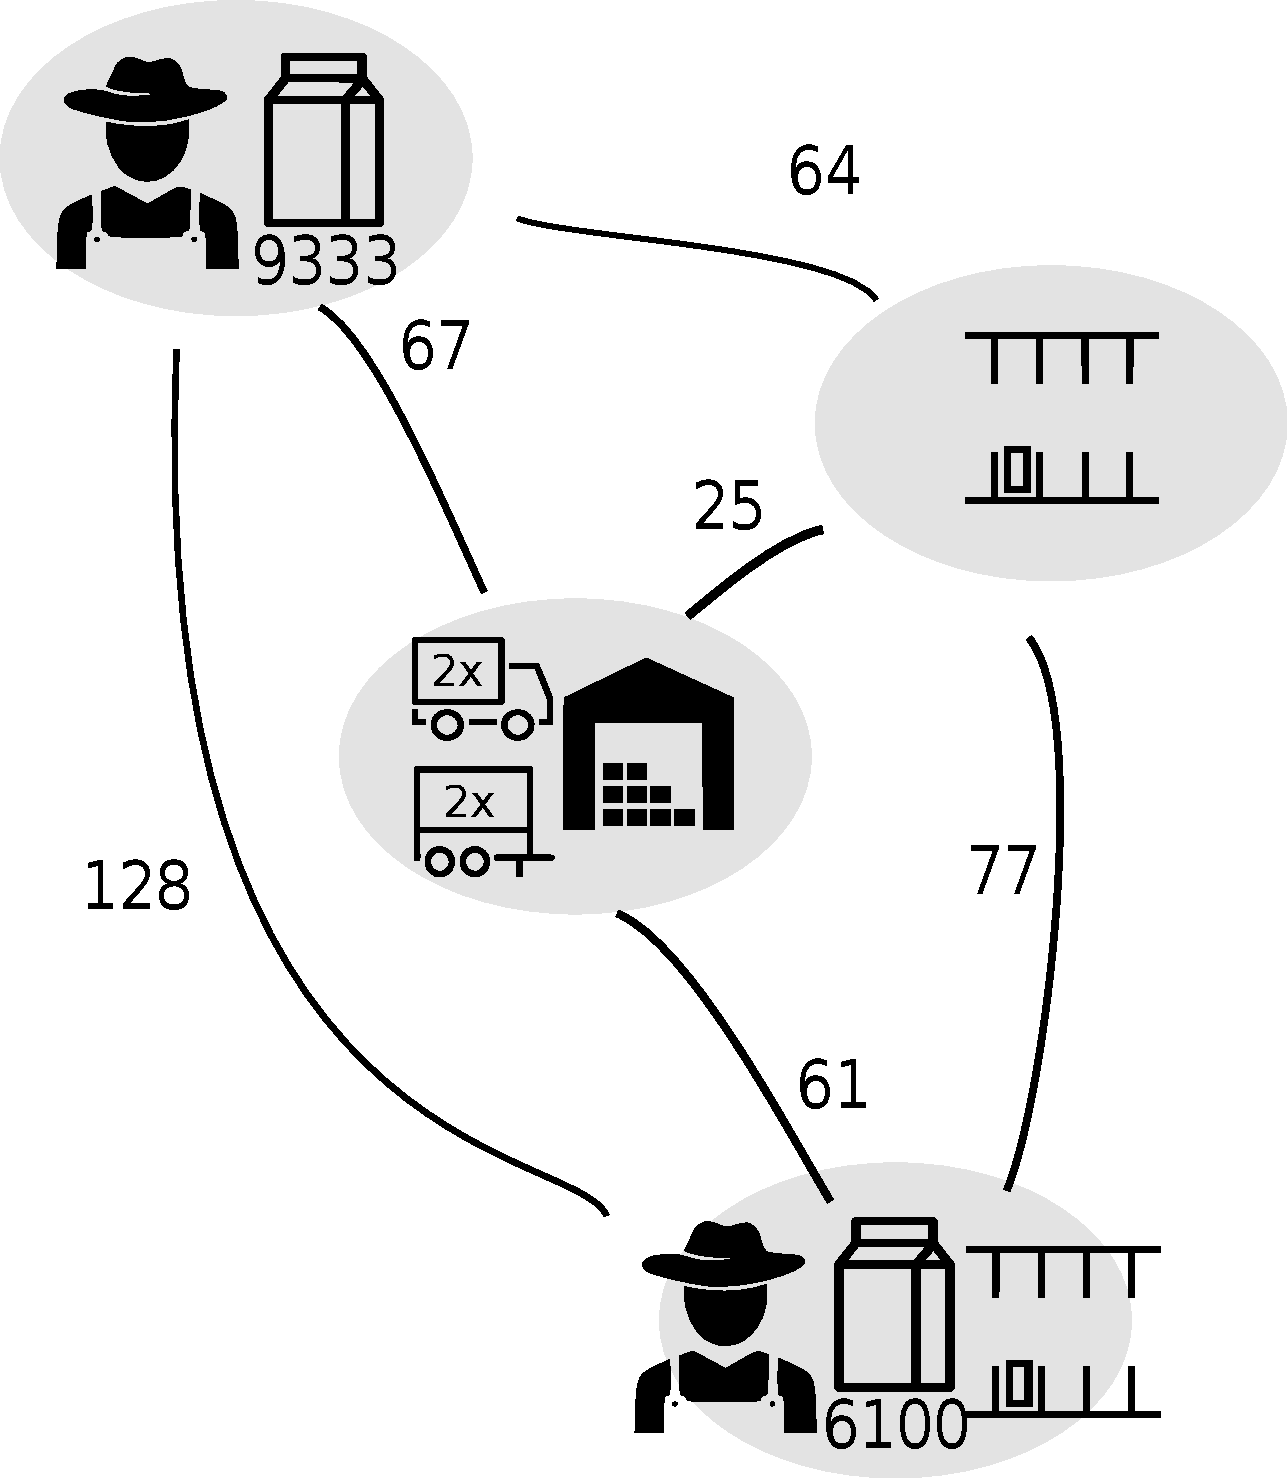
\includegraphics[width=.8\textwidth]{img/1_1_1_4.pdf}
  \caption{Instance $1\_1\_1\_4$ which consist of a depot, a lorry customer, a trailer customer and a pure transshipment location. The distance is in kilometers and the numbers at the customers' is the amount of their supply. The fleet consists of one of each of the vehicles described in Table \ref{tab:vehpar}. }
  \label{fig:instance}
\end{figure}

An example of the benefits of allowing lorries to do multiple trips is given in Figure  \ref{fig:instance}. It illustrates one of the instances with two customers. The fleet consist of one of each of the vehicles described in Table \ref{tab:vehpar}. There is a lorry customer with a supply of 9333 units, a trailer customer with a supply of 6100 units and a pure transshipment location. The time window of each location is the interval [0 , 1320] minutes hence there is enough time for one lorry to visit both customers and collect their supplies.
The sum of the customer supplies is equal to 15433 which is bigger than the capacity of either lorry.
If the lorry is allowed to do multiple trips, it can unload at the depot between visiting the customers.
If this is not allowed, the cheapest solution is to use a trailer.
The fixed cost of this trailer will need to be paid together with its distance related costs.
In Appendix \ref{sec:gaps} we can see that allowing lorries to do multiple trips leads to a gap of -13.8 \% with respect to the optimal value of the TTRP including time costs and -12.5 \% with respect to the optimal value of the VRPTT excluding time costs for this instance.

 % \begin{figure}[h]
 %    %  \makebox[\textwidth][r]{\includegraphics[width=1.2\textwidth]{img/results_multiple_unload.png}}%
 %  %  \centering
 %  % \includegraphics{...}}
 %  % \hspace*{-1.5in}
 %  % \centerline{\includegraphics{...}}
 %     \includegraphics[width=1.\textwidth]{img/results_multiple_unload.png}
 %   \caption{The lowest found costs for the VRPTT with and without time related costs are plotted. Bounds for the TTRP with time related costs and bounds for  the VRPTT without time related costs are given.  Constraint \eqref{con:extra} does not hold. The instances are ordered for a better presentation. }
 %   \label{fig:single_unload}
 % \end{figure}


%  In Figure \ref{fig:single_unload} we see the same bounds, but this time our results represent the best found values without constraint (\ref{con:extra}). For all instances feasible solution could be found. Being able to unload multiple times has significantly reduced costs. When time related costs are included the average gap between  our best solution, and the optimal solution of the TTRP is $ -8.0\%$.
%
% If we exclude time related costs the average gap between the lower (higher) bound and our best solution is $ -11.7\% (-14.0\%)$ .
%
%
%
% %
%
%
%
%
%
%
% \subsection{usefulness multi unload}
% A simple example that illustrates the advantage of being able to unload multiple times is shown in Figure \ref{fig:instance}



% The depot has two available lorries and two available trailers. There are two customers that lie far apart. The vehicles have a speed of 65 kilometers per hour. The time windows of the locations start at 0:00 hours and end at 20:00 hours, so there is more than enough time for a lorry to visit both customers. One lorry has a capacity of 10000 and the other has a capacity of 15000. One trailer has a capacity of 10000 and the other has a capacity of 15000. If constraint (\ref{con:extra}) holds, either two lorries , or a lorry and a trailer have to be used. If the constraint is removed, the cheapest lorry can be used to visit both customers without using a trailer by unloading at the depot before going to the second customer.
%





% % \usepackage{booktabs}
% \newcommand{\ra}[1]{\renewcommand{\arraystretch}{#1}}
% \begin{table*}\centering
% \ra{1.3}
% \begin{tabular}{@{}rrrrcrrrcrrr@{}}\toprule
% & \multicolumn{3}{c}{$w = 8$} & \phantom{abc}& \multicolumn{3}{c}{$w = 16$} &
% \phantom{abc} & \multicolumn{3}{c}{$w = 32$}\\
% \cmidrule{2-4} \cmidrule{6-8} \cmidrule{10-12}
% & $t=0$ & $t=1$ & $t=2$ && $t=0$ & $t=1$ & $t=2$ && $t=0$ & $t=1$ & $t=2$\\ \midrule
% $dir=1$\\
% $c$ & 0.0790 & 0.1692 & 0.2945 && 0.3670 & 0.7187 & 3.1815 && -1.0032 & -1.7104 & -21.7969\\
% $c$ & -0.8651& 50.0476& 5.9384&& -9.0714& 297.0923& 46.2143&& 4.3590& 34.5809& 76.9167\\
% $c$ & 124.2756& -50.9612& -14.2721&& 128.2265& -630.5455& -381.0930&& -121.0518& -137.1210& -220.2500\\
% $dir=0$\\
% $c$ & 0.0357& 1.2473& 0.2119&& 0.3593& -0.2755& 2.1764&& -1.2998& -3.8202& -1.2784\\
% $c$ & -17.9048& -37.1111& 8.8591&& -30.7381& -9.5952& -3.0000&& -11.1631& -5.7108& -15.6728\\
% $c$ & 105.5518& 232.1160& -94.7351&& 100.2497& 141.2778& -259.7326&& 52.5745& 10.1098& -140.2130\\
% \bottomrule
% \end{tabular}
% \caption{Caption}
% \end{table*}


% \newpage
% \input{real_values.tex}


% plot here:
% violin plot.
%
% 1 x value for each instance size group.
% left size is for
%
% Give the plot such that I can say:
% we see that our algo does not find results as good as the ttrp algo. This can have 2 reason either they are there but hte algo does not find them, or no better sols exist and therefore they are not found. Looking at the figures, we see that the

% \subsubsection{VRPTT Instances}
% Drexl's instances used in \cite{drexl2014bandc} with up to 8 requests have been used to test the algorithm.
%
% \begin{table}[ht]
% \centering
% \caption{My caption}
% \label{my-label}
% \begin{tabular}{llllll}
% \hline
%                 & Capacity             & Fixed costs & Costs per km & Driving speed & $C_k$ \\ \hline \hline
% Lorry class 1   & 10000              & 180    & 0.65       & 65            & $\{1,2\}$                        \\ \hline
% Lorry class 2   & 15000                & 200    & 0.7        & 65            & $\{1\}$                          \\ \hline
% Trailer class 1 & 10000       & 20     & 0.04       &               &  $\{1,2\}$                          \\ \hline
% Trailer class 2 & 15000          & 25   & 0.04          &               &   $\{1\}$                         \\ \hline
% \end{tabular}
% \end{table}
%
% \todo{add details about parameters}
%
% \subsubsection{TTRP Instances}
% Drexl's instances with up to 25 requests used for the truck-and-trailer routing problem in  \cite{drexl2011branch}.
%
% \subsection{Results}
% In the table below  we can observe \ldots
% \subsection{Usefulness Trailer Sharing}
